\chapter{NEAT Boundary Layer Wind Tunnel}

%%%%%%%%%%%%%%%%%%%%%%%%%%%%%%%%%%%%%
%%%%%%%%%%%%%%%%%%%%%%%%%%%%%%%%%%%%%
\section{Experimental Facility}

\begin{figure}[h!]
\centering
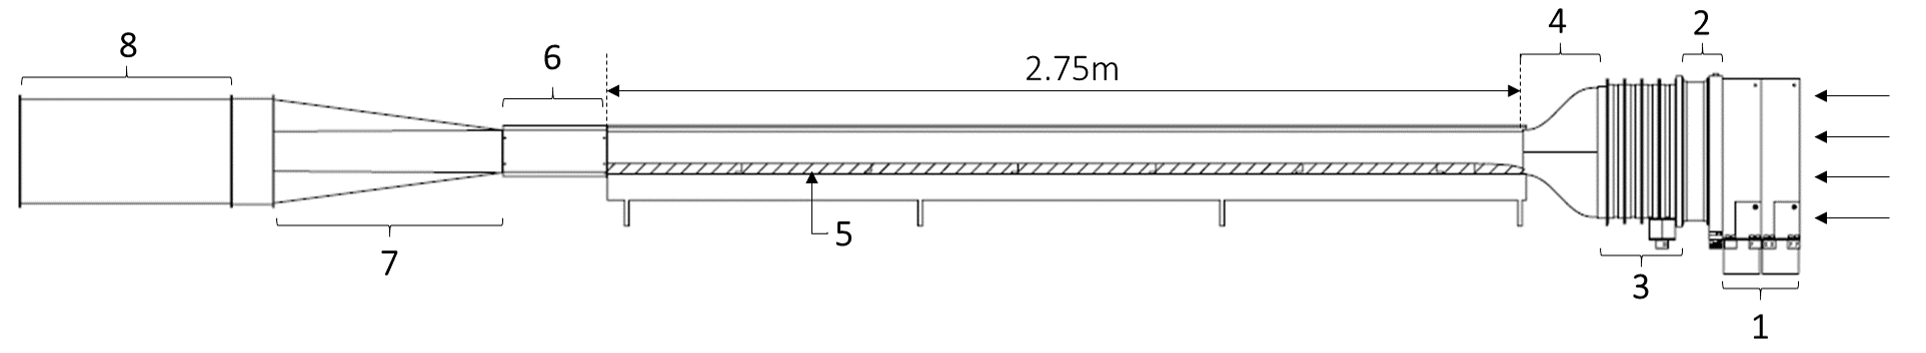
\includegraphics[scale=.45]{facility/tunnel_v7.png}
\caption{Schematic of the experimental facility. Air enters the facility from right-to-left. The primary components include: (1) freestream heaters, 
(2) seeding manifold, (3) turbulence management section, (4) contraction, (5) thermal wall-plate located on the bottom wall of the test-section, (6) rotor-stator assembly, (7) diffuser, (8) centrifugal fan.}
\label{fig:tunnel}
\end{figure}

The NEAT boundary layer wind tunnel is an open-circuit in-draft type designed to study heat transfer in non-equilibrium boundary layers. Figure ~\ref{fig:tunnel} shows the design schematic for the facility. The key design component is the thermal wall plate used to control the lower-wall thermal boundary conditions seen by the flow. 

%%%%%%%%%%%%%%%%%%%%%%%%%%%%
\subsection{General Description}
%provide back to front overview of tunnel, then pull each piece and describe in more detail
The inlet section to the tunnel consists of a feed-back controlled resistive heater bank, a seeding manifold, a turbulent management section and a 4:1 contraction. 
The test-section of the tunnel nominally measures 303mm $\times$ 111mm cross-section and 2.75m in length and is made of plexiglass to allow optical access.
Removable windows in the top wall of the tunnel sit at 45, 136.3, and 251.8 cm from the test section inlet which allow for the introduction of probes, laser light, or IR measurements into the tunnel test section 
A feed-back controlled thermal wall-plate sits on the floor of the test section and is used to control the lower-wall temperature seen by the flow. 
The leading edge of the thermal wall-plate is a super-ellipse designed to prevent flow separation \cite{R.Narasimha1994}. 
The upper wall of the test-section is angled at 0.23$^\circ$ to closely maintain a ZPG condition along the length of the test-section. 
Downstream of the test-section is a pulsatile flow generator used to produce a sinusoidal pressure gradient, creating a non-equilibrium flow condition. 
The diffuser transitions the flow area from a rectangular to a circular cross-section where it connects to a belt driven centrifugal fan.  
A frequency controller is used to control and maintain the fan speed and corresponding flow speed in the test-section. 
The freestream velocity in the test-section can vary between 1 and 12$ms^{-1}$. 
The entire tunnel sits on a custom frame which levels and isolates the tunnel test-section.
In the following subsections, the components of the facility are described in detail.


%%%%%%%%%%%%%%%%%%%%%%%%%%%%%%%%%%%%
\subsection{Inlet Section}
%discuss heaters, seeder, turb managment, contraction
%Heater%

Air entering the test-section first passes through an OMEGA Engineering air duct heater (model CABB-1211/208). 
The 3-phase 208V heater consists of nine sheathed finned chrome steel resistive heaters that provide 12 kW of power (with a power density of 4.03 W/cm$^2$). 
The cross-sectional area of the heater is 390.5mm $\times$ 358.8mm with an open area of 859.4 cm$^2$ (blockage of about 39\%). 
The three legs of the AC power are connected to the heater through a Watlow Din-A-Mite C silicone controller rectifier (SCR) power controller. 
A type J thermocouple placed in the freestream 1m downstream of the test-section inlet provides feedback for a proportional, integral, and derivative (PID) controller used as the input for the SCR power controller. 
The SCR power controller, configured for zero-voltage crossover firing (as opposed to phase angle crossover firing) to reduce electrical noise, is used to regulate the duty cycle of the voltage (either 0\% or 100\%) to the heaters thereby controlling the freestream temperature. 
A SCR power controller was chosen (over a mechanical relay or solid state relay) as it is more suitable for handling the large current (33.4A) needed for the heater and has a fast response time of 5.56ms, which not only allows for a tightly controlled freestream temperature but also prolongs the life of the heating elements by reducing the thermal fatigue.

The PID controller gains are optimized for varying freestream velocity and temperature conditions, as one set of gain values does not work well over a large operating range. 
This is achieved using the autotune feature of the SCR power controller-PID feedback system. 
The ability of the system to hold a freestream set point temperature is shown in Fig.~\ref{fig:inlet}(a). 
%Seeder%
After exiting the heater, the air flow passes through a honeycomb-type seeding manifold to introduce (if desired) tracer particles into the flow to be used for particle image velocimetry (PIV).
The challenge with seeding an open-circuit wind tunnel is that the flow tracers must be uniformly distributed into the flow at the source. 
This is much more difficult than seeding a closed-circuit wind tunnel where the seed can be allowed to circulate through the facility to produce a uniform seed concentration. 

\begin{figure*}[t!]
  \begin{center}
  {\subfigcapskip = -20pt \subfigcapmargin = -12pt \subfigure[]{\label{fig:edge-a}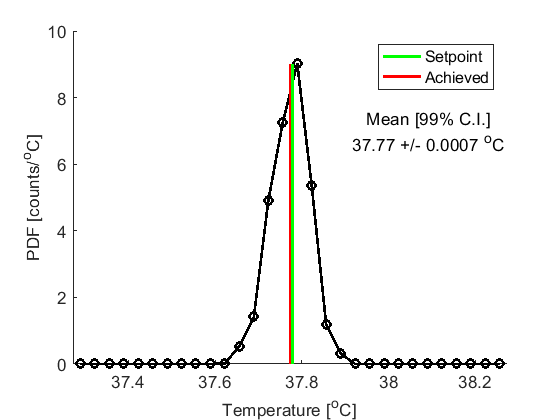
\includegraphics[scale=0.45]{facility/HeatCI_4mps100F_v3.png}}}
   {\subfigcapskip = -20pt \subfigcapmargin = -12pt  \subfigure[]{\label{fig:edge-b}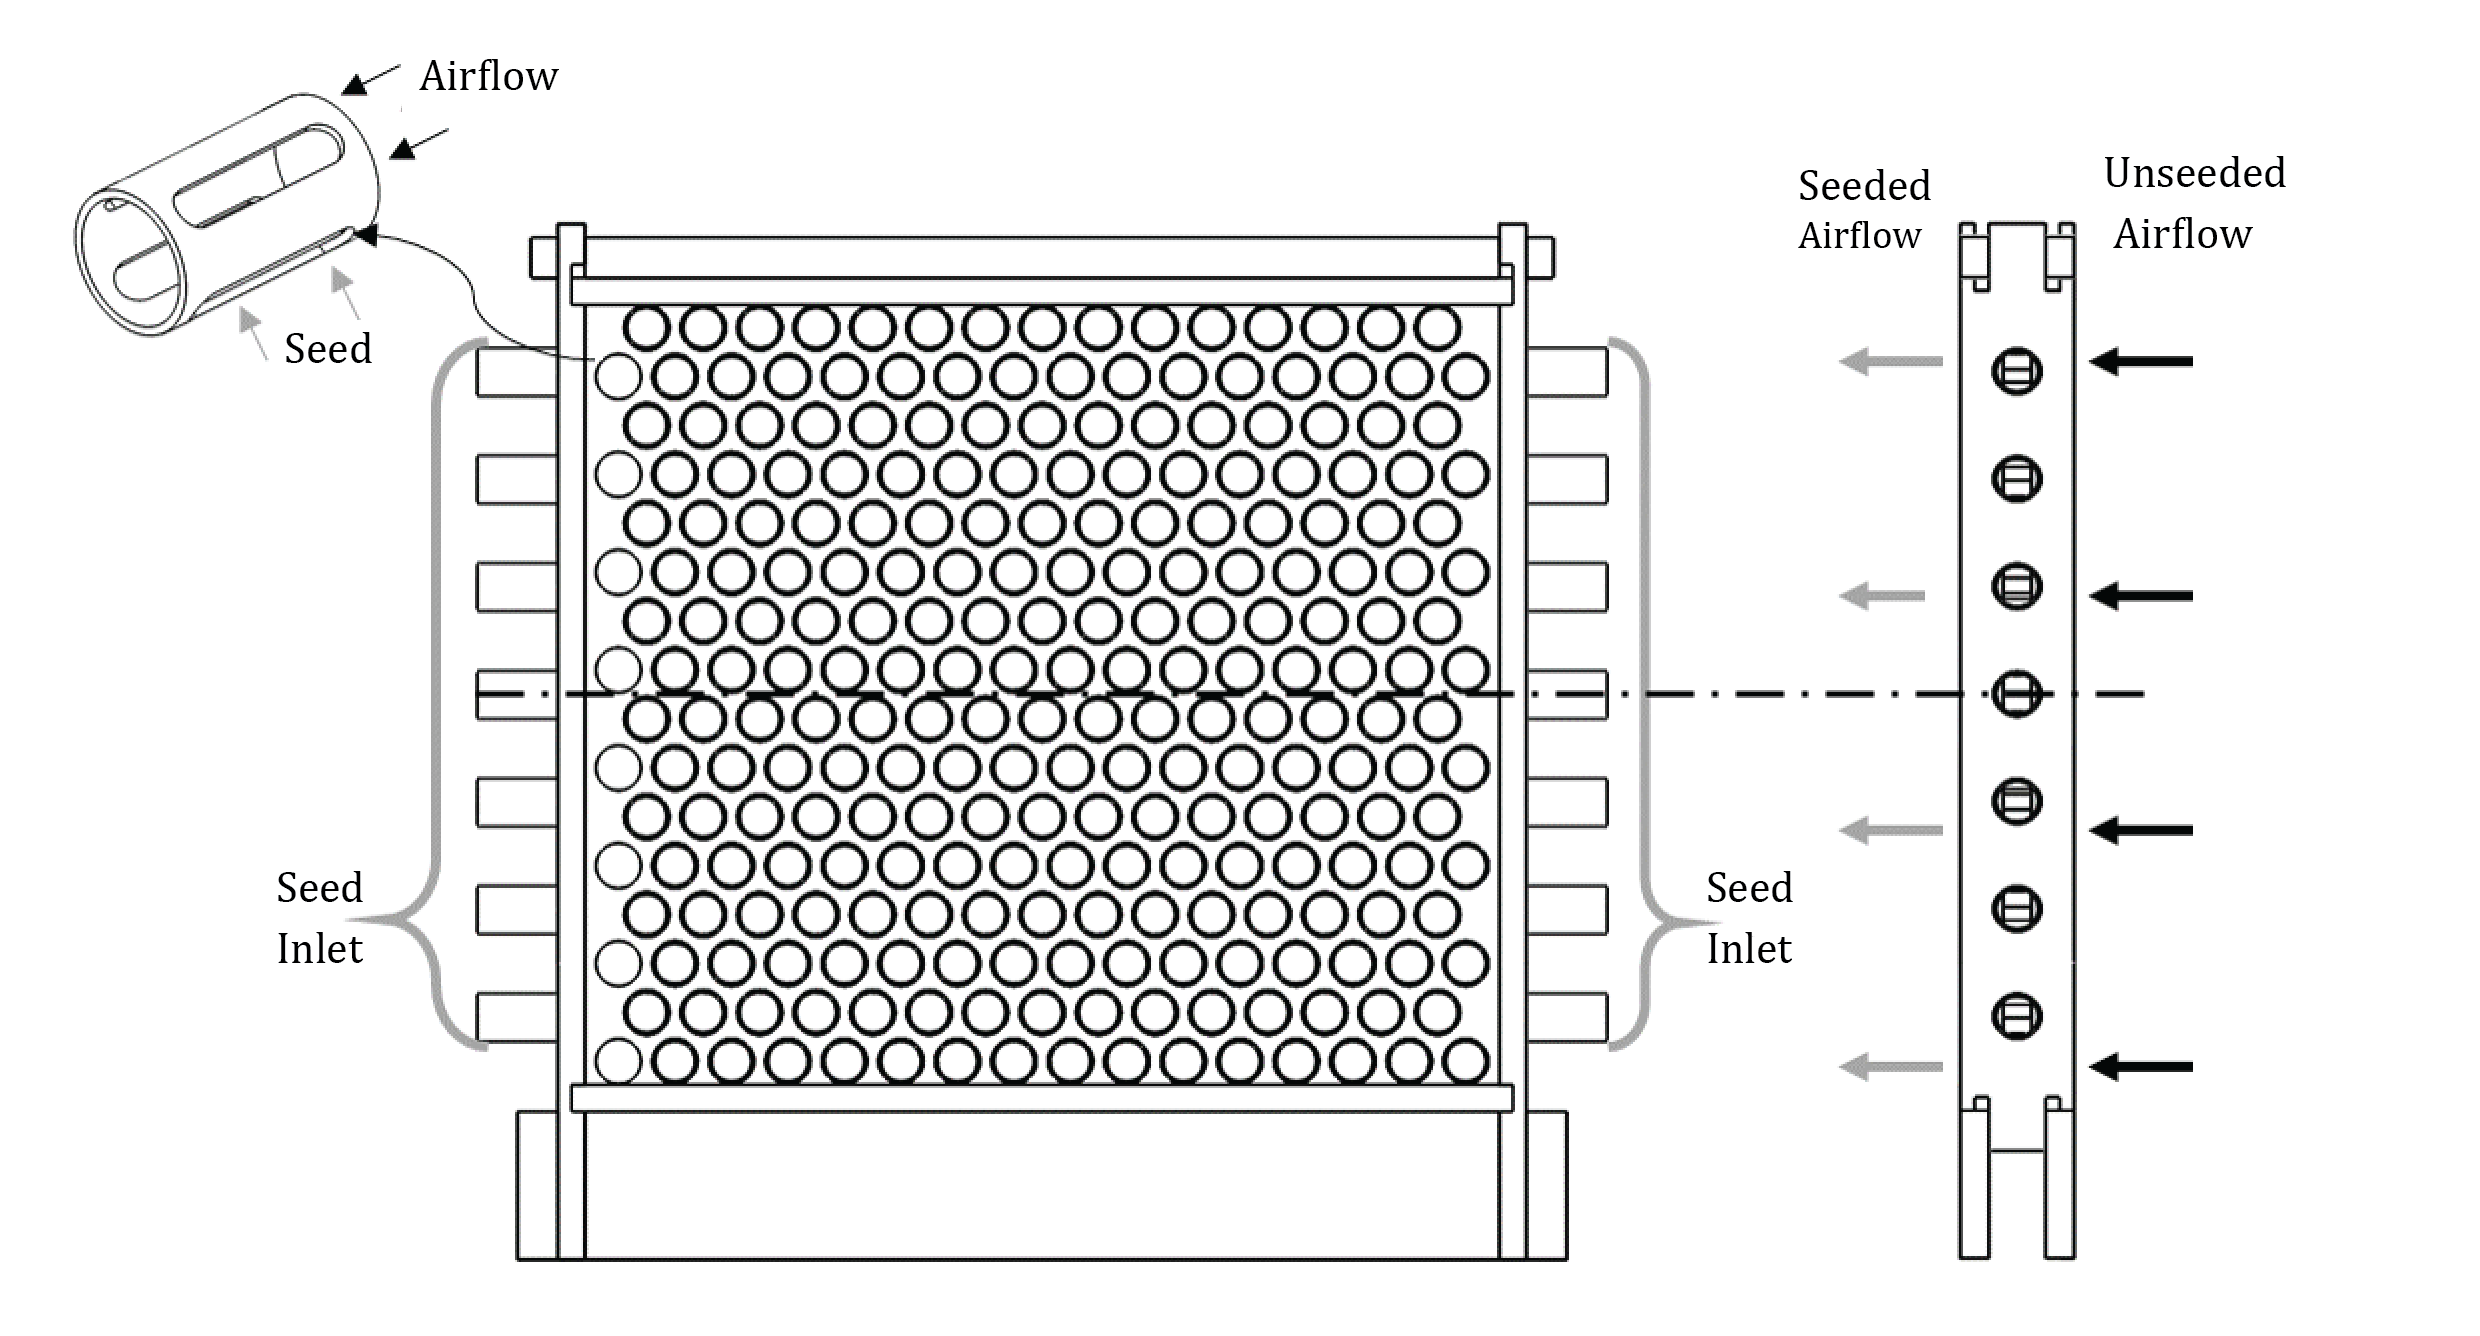
\includegraphics[scale=0.4]{facility/seeding_manifold_v2.png}}}
  \end{center}
 \caption{\label{fig:Virk_model} \footnotesize (a) Probability density function (PDF) of freestream temperature measured in the wind tunnel over a two hour period. The vertical green line represents the setpoint temperature and the vertical red line represents the measured mean temperature with a confidence interval of 99\%. (b) Schematic of the seeding manifold used for particle image velocimetry (PIV).}  
\label{fig:inlet}
\end{figure*}

The custom designed seeding manifold is shown in Fig.~\ref{fig:inlet}(b). 
The inlet air flows across the manifold through 248 PVC tubes of length 38.1mm and diameter 21.34mm. 
Four slots of 25.4mm length and 6.35mm width separated by 90$^\circ$ (center-to-center) are cut into each PVC tube. 
The plenum volume of the seeding manifold is filled with a dense fog of nominal 1$\mu$m  diameter oil droplets \cite{Shakerin1995} through up to twenty-three 21.34mm diameter pipes mounted around the perimeter of the seeder connected to a ROSCO 1700 fogger. 
The fog is drawn into the PVC inlet air piping through the four slots owing to the pressure difference between the fog in the plenum and the air in the PVC tubes. 
The open area percentage of the manifold (56.5\%) is comparable to the open area of the freestream heater (61\%). 
Detailed drawings of the seeding manifold can be found in App.~\ref{sec:draw}.
%Turb Management-contraction%
%drawings on contraction? any more info to add?
The air then passes through a turbulence management section containing 4 screens of decreasing wire mesh size and then a honeycomb section.
The screens reduce axial turbulence while the honeycomb reduces lateral turbulence.
The air flow then proceeds through a 4:1 contraction to speed up the flow and to further reduce turbulent intensities.

%%%%%%%%%%%%%%%%%%%%%%%%%%%%%%%%%%%%
\subsection{Test Section}
%discuss trip, window design, tunnel frame

\begin{figure}[h!]
\centering
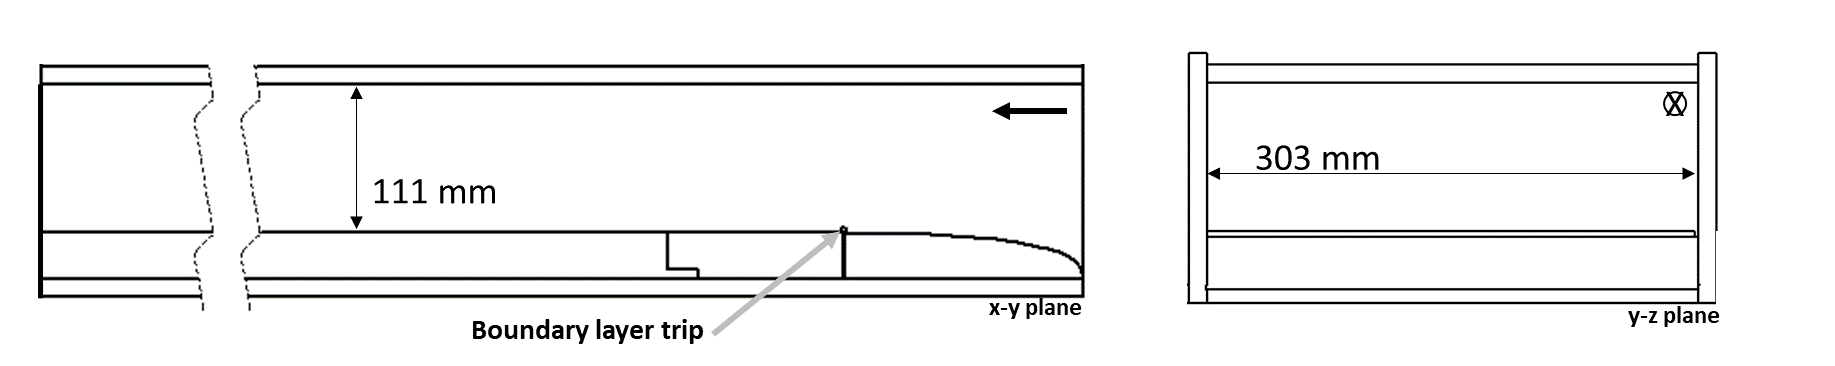
\includegraphics[scale=.45]{facility/testSectionV1.png}
\caption{\footnotesize Does this look to small or is the other size better}
\label{fig:testSection}
\end{figure}

%Trip
To investigate turbulent boundary layers, a 3mm diameter trip rod extending the spanwise extent of the test-section is placed on the rear of the leading-edge nose, just upstream of the first convective plate.
The rod induces transition to turbulence and fixes (on average) the starting location of a developing turbulent boundary layer.
A range of trip diameters as well as shape were tested to determine the smallest diameter which would lead to a steady (on average) transisition. 
An undersized trip does not induce enough energy and the flow can relax back to a laminar state, while too large of a trip produces near wall effects which do not decay in an appropriate range \cite{Marusic2015}.
Wall normal velocity profiles taken at the first measurement location verified the appropriate trip diameter by comparing mean profiles as the recovery length does not depend on the order of the statistic measured \cite{Marusic2015}.

%Window Inserts%
\begin{figure}[h!]
\centering
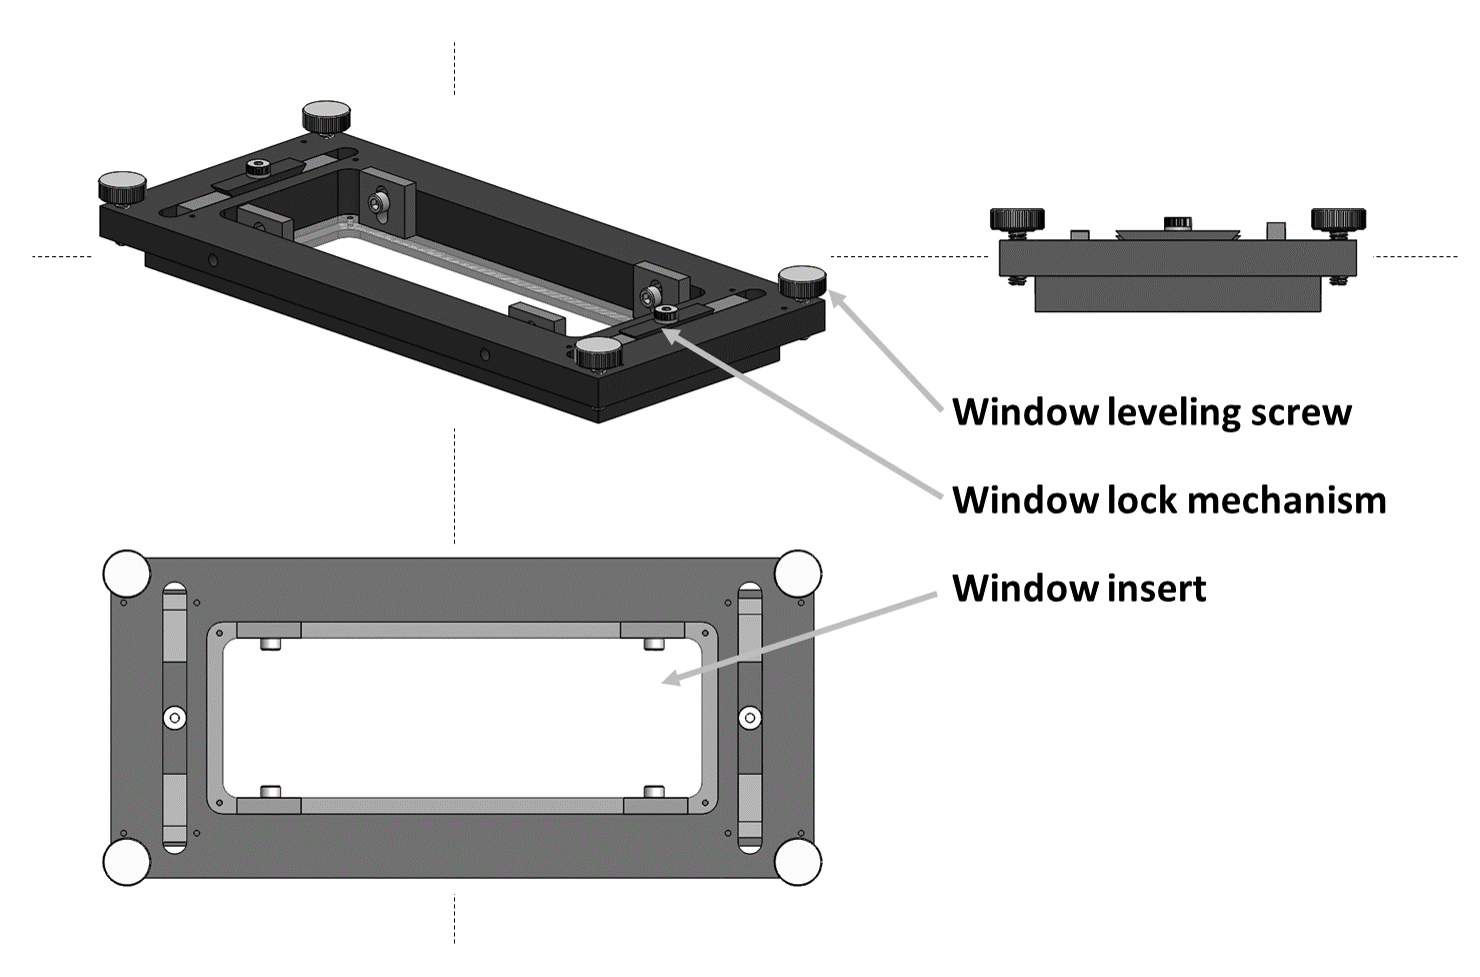
\includegraphics[scale=.45]{figures/facility/tunnelwindows.png}
\caption{Schematic of removable windows which allow for optical measurements and installation of temperature/velocity probes. Design was developed by Dr. Michael Allard}
\label{fig:tunnelWindow}
\end{figure}

Three windows of size 254mm $\times$ 102mm sit in the top wall of the test-section located at approximately 45, 136.3, and 251.8cm from the test-section inlet.
The windows are used for introduction of laser light, for infrared (IR) imaging and for inserting various measurement probes.
The window body, seen in Fig.~\ref{fig:tunnelWindow}, contains 4 leveling screws such that window can be set flush with the inside wall of the tunnel.
Window inserts made from either BK7 glass of clear poly-carbonate can be installed depending on the requirement.
The optical quality of the glass inserts are better than the plexiglass walls and necessary for IR imaging.
%tunnel frame
The tunnel frame, which supports the working section of the tunnel, has leveling adjustments in the x and z direction such that the tunnel floor sits parallel to the adjacent optics table. 
This then orients the x-y plane of the tunnel and any optical equipment mounted to the optical table.
Custom optics mounting boards line the streamwise length of the tunnel for ease of experimental setup.
The entire frame sits on damping feet which isolate the tunnel from any ambient vibrations in the room.

%%%%%%%%%%%%%%%%%%%%%%%%%%%%%%%%%%%%%%%%%%
%%%%%%%%%%%%%%%%%%%%%%%%%%%%%%%%%%%%%%%%%%
\section{Thermal Wall-plate}
\subsection{Prototype Wall-plate}
%discuss prototype design, manufacturing, final design
%include drawings in appendix (ref=sec:designdraw)
The thermal wall plate covers the bottom floor of the NEAT test section and controls the bottom wall boundary condition by setting $T_{wall}$.
The design is modeled after the work of Blackwell et al. \cite{Blackwell1972}.
The base design consists of a thermal mass which is heated and maintained at a set temperature.
The main design condition was that the system must be able to maintain a set wall temperature independent of the above flow state (i.e. 2-D varying wall heat flux).
Other design constraints were to minimize the height of the system so as to reduce blockage effects; minimize conductive heat loss from the thermal mass so as to ensure all heat was going into convective transfer; and to design a system which could be manufactured in house and installed with ease into the NEAT tunnel.

For prototype development a different open circuit down draft wind tunnel was used as it had a smaller development length and had a greater ease of access to the working section.
The working section of the tunnel is 0.45m x 0.45m x 0.66m (z by y by x).
To account for the streamwise variation in heat flux (coming from a developing boundary layer) the prototype design consisted of two convective plates with increasing streamwise length based on downstream location.
This also assisted in ease of manufacturing as the parts could then fit within the working area of the UNH machine shop.\\

\begin{figure}[h!]
\centering
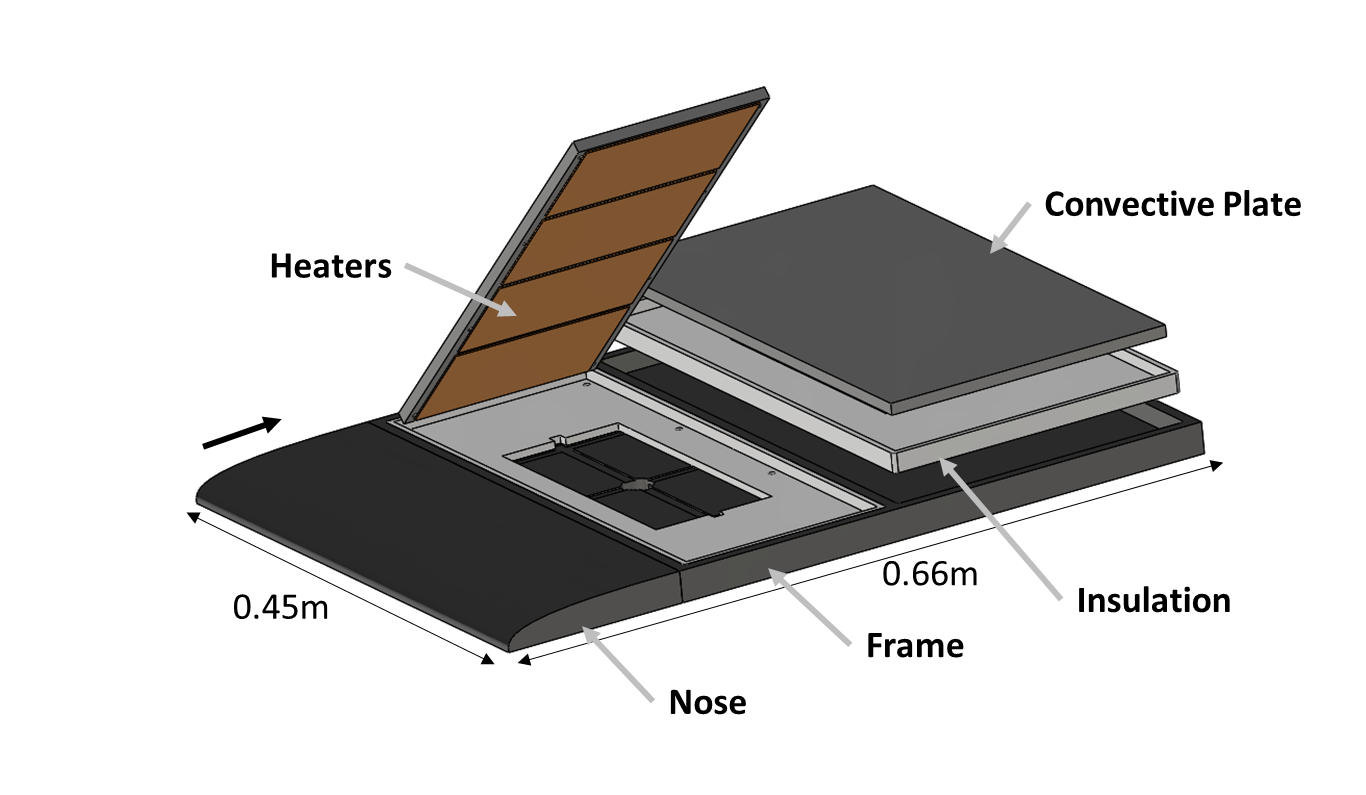
\includegraphics[scale=.45]{facility/prototypePlateV1.png}
\caption{\footnotesize Solid model of prototype thermal wall plate with two convective plates.} 
\label{fig:prototype}
\end{figure}

Fig.~\ref{fig:prototype} shows the solid model design of the prototype thermal wall plate.
The convective plate is an aluminum 6061 plate which is 9.5mm thick.
For heating the Al plate, there is an array of Kapton polyimide-fllm resistive resistive heaters (affixed to the bottom of the aluminum plate) with a heating density of 1.5W/cm$^2$.
In between the heaters there are a series of holes which contain J-type thermocouples, which then sit 2.5mm beneath the surface of the plate and act in a feed back loop to control the convective plate temperature.
Each Al plate sits into a custom machined section of insulation made from calcium-silicate.
Each of the insulated wall plates then sit into a frame manufactured from Delrin which sets the spacing of each plate, and was chosen for its low thermal conductivity and machinability.
Due to the desire of producing high quality physics grade boundary layers a leading edge nose was developing to smoothly transition the flow onto the thermal wallplate.
The nose utilizes a super-ellipse design to prevent flow separation \cite{R.Narasimha1994} which was determined according to Eqn. 1 of Narasimha et al;

\begin{equation}
[(a-x)/a]^2 + (y/b)^2 = 1
\label{eq:superEllipse}
\end{equation} 

where x is the streamwise position, y is the wall normal position, a is the length of the nose, 2b is the height of the nose.
To accurately recreate the desired profile a three-axis controlled CNC machine was used to smoothly cut the profile into the Delrin.
Fig.~\ref{fig:nose} shows the fabrication process applied to the final implemented design.

The prototype design was used for testing and developing wall temperature control schemes.
A variety of measurements were made with the plate including; ZPG wall temperature distribution, and wall temperature distribution due to wake behind a hemisphere.
The ZPG conditions validated the base design and demonstrated that ZPG thermal boundary layer developed as expected when compared to literature.
The wake study gave insight into the performance of the design in complex flow states.
It was found that future designs should utilize spanwise oriented bottom heaters as streamwise oriented heaters require individual zone control, where multiple controllers would be used to control the temperature of a single plate.
The final design for installation into the NEAT tunnel incorporates many lessons learned from the prototype plate such as from manufacturing limits, material limits, and ease of operation and repair.

%%%%%%%%%%%%%%%%%%%%%%%%%%%%%%%%%%%%
\subsection{Finalized Wall-plate}

\begin{figure}[h!]
  \begin{center}
  {\subfigcapskip = -20pt \subfigcapmargin = -12pt \subfigure[]{\label{fig:edge-a}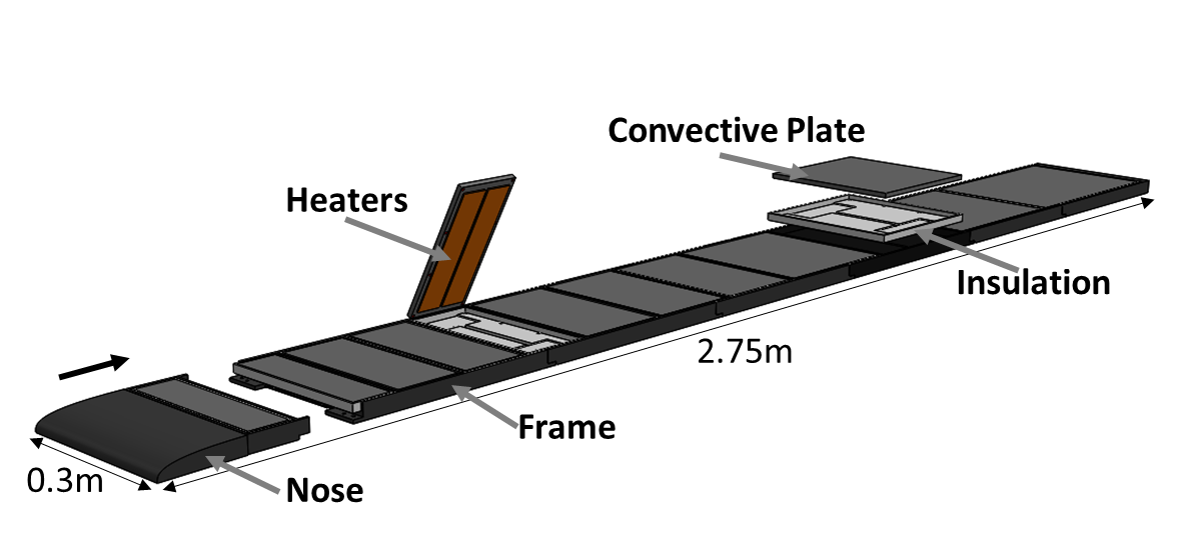
\includegraphics[scale=0.5]{figures/facility/wallplate_SW.png}}}
   {\subfigcapskip = -20pt \subfigcapmargin = -12pt  \subfigure[]{\label{fig:edge-b}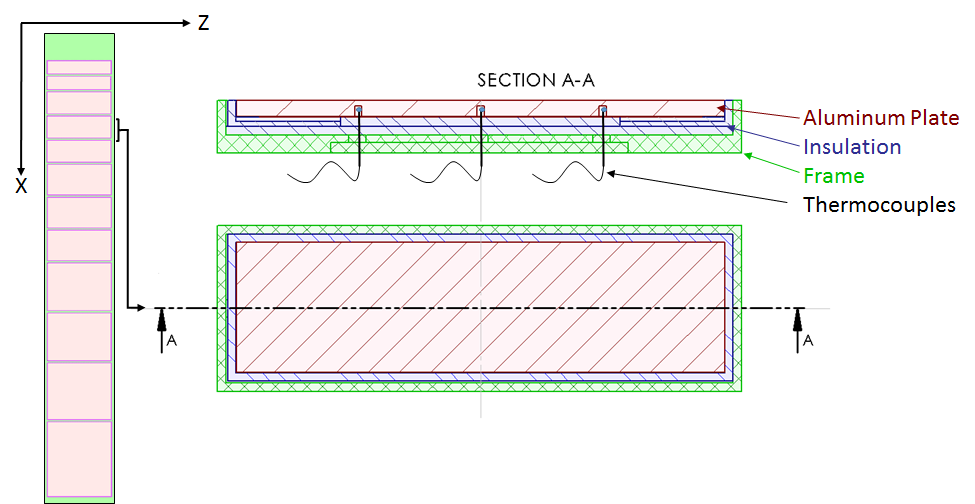
\includegraphics[scale=0.4]{figures/facility/plate_setup_sketch_v5.png}}}
  \end{center}
 \caption{\label{fig:Virk_model} (a) Solid model schematic of the thermal wall-plate. (b) Detailed schematic of a section of the thermal wall-plate: right tilted 45$^o$ lines denotes the heated wall plate, left tilted 45$^o$ lines shows the surrounding layer of calcium silicate insulation and the hash marked section represents the co-polymer acetal frame which positions all components. Three evenly spaced embedded thermocouples are located along line $AA$.}  
\label{fig:wallplate}
\end{figure}

The final thermal wall-plate (shown in Fig.~\ref{fig:wallplate}) comprises of twelve sections each independently heated and controlled. 
Each section consists of a 9.5mm thick aluminum 6061 plate, Kapton polyimide-fllm resistive resistive heaters (affixed to the bottom of the aluminum plate) with a heating density of 1.5W/cm$^2$, and a 5mm thick calcium silicate holder used for thermal isolation of the aluminum plate (the thermal conductivity of the calcium silicate is four-orders of magnitude less the aluminum 6061).
Three evenly spaced J-type thermocouples arranged spanwise in the center of each plate and embedded 2.5mm beneath the top surface of each aluminum plate are used to monitor wall temperature for feedback control of wall heating. 
To increase ease of assembly and repair a thermocouple holder was designed to maintain the position of each thermocouple throughout assembly and operation.
To ensure each thermocouple had adequate contact with the convective plate, each thermocouple hole was filled with a silver grease compound which is thermally conductive and electrically insulative.
The section components sit in a Delrin (acetal) frame, which incorporates a method of leveling each section indivdually such that the overall surface roughness of the assembly can be reduced.
The streamwise (flow direction) length of each section increases with downstream position such that the convective heat transfer from plate-to-plate does not vary by more than a suitably chosen threshold of 15\%.
This threshold is set by examining the smallest feasibly manufacturable streamwise plate length of the most upstream plate, as this is where the heat flux changes most rapidly. 
The length of the plates are summarized in Table~\ref{tab:plate}. 

\begin{table}[t!] 
\centering
\caption{\indent The length of the convective plates. Plate 1 is at the upstream end and plate 12 is at the downstream end of the wind tunnel.}
%\resizebox{\columnwidth}{!}
\label{tab:plate}
\end{table}

For ease of manufacturing the streamwise length of the plates stayed consistent for 2-3 adjacent plates.
This made for the manufacturing of similar components which sped up the process and kept the streamwise length of progressing plates smaller which assist with better boundary condition control.
The entire wall plate system was design in a manor such that it could be assembled/disassembled with only one person. 
Interlocking frame sections are custom fit to within -.127 +0 mm of the tunnel width such that the system can be assembled plate by plate and slid into the tunnel from the inlet.
Routed wires for heater power and thermocouple output are fed out of bottom windows which match the position of the top windows.
Detailed descriptions and drawings of the individual wall-plate components as well as description of the assembly and installation process can be found in App.~\ref{sec:NEATcomponents}.

\begin{figure}[h!]
  \begin{center}
  {\subfigcapskip = 5pt \subfigcapmargin = -12pt \subfigure[]{\label{fig:edge-a}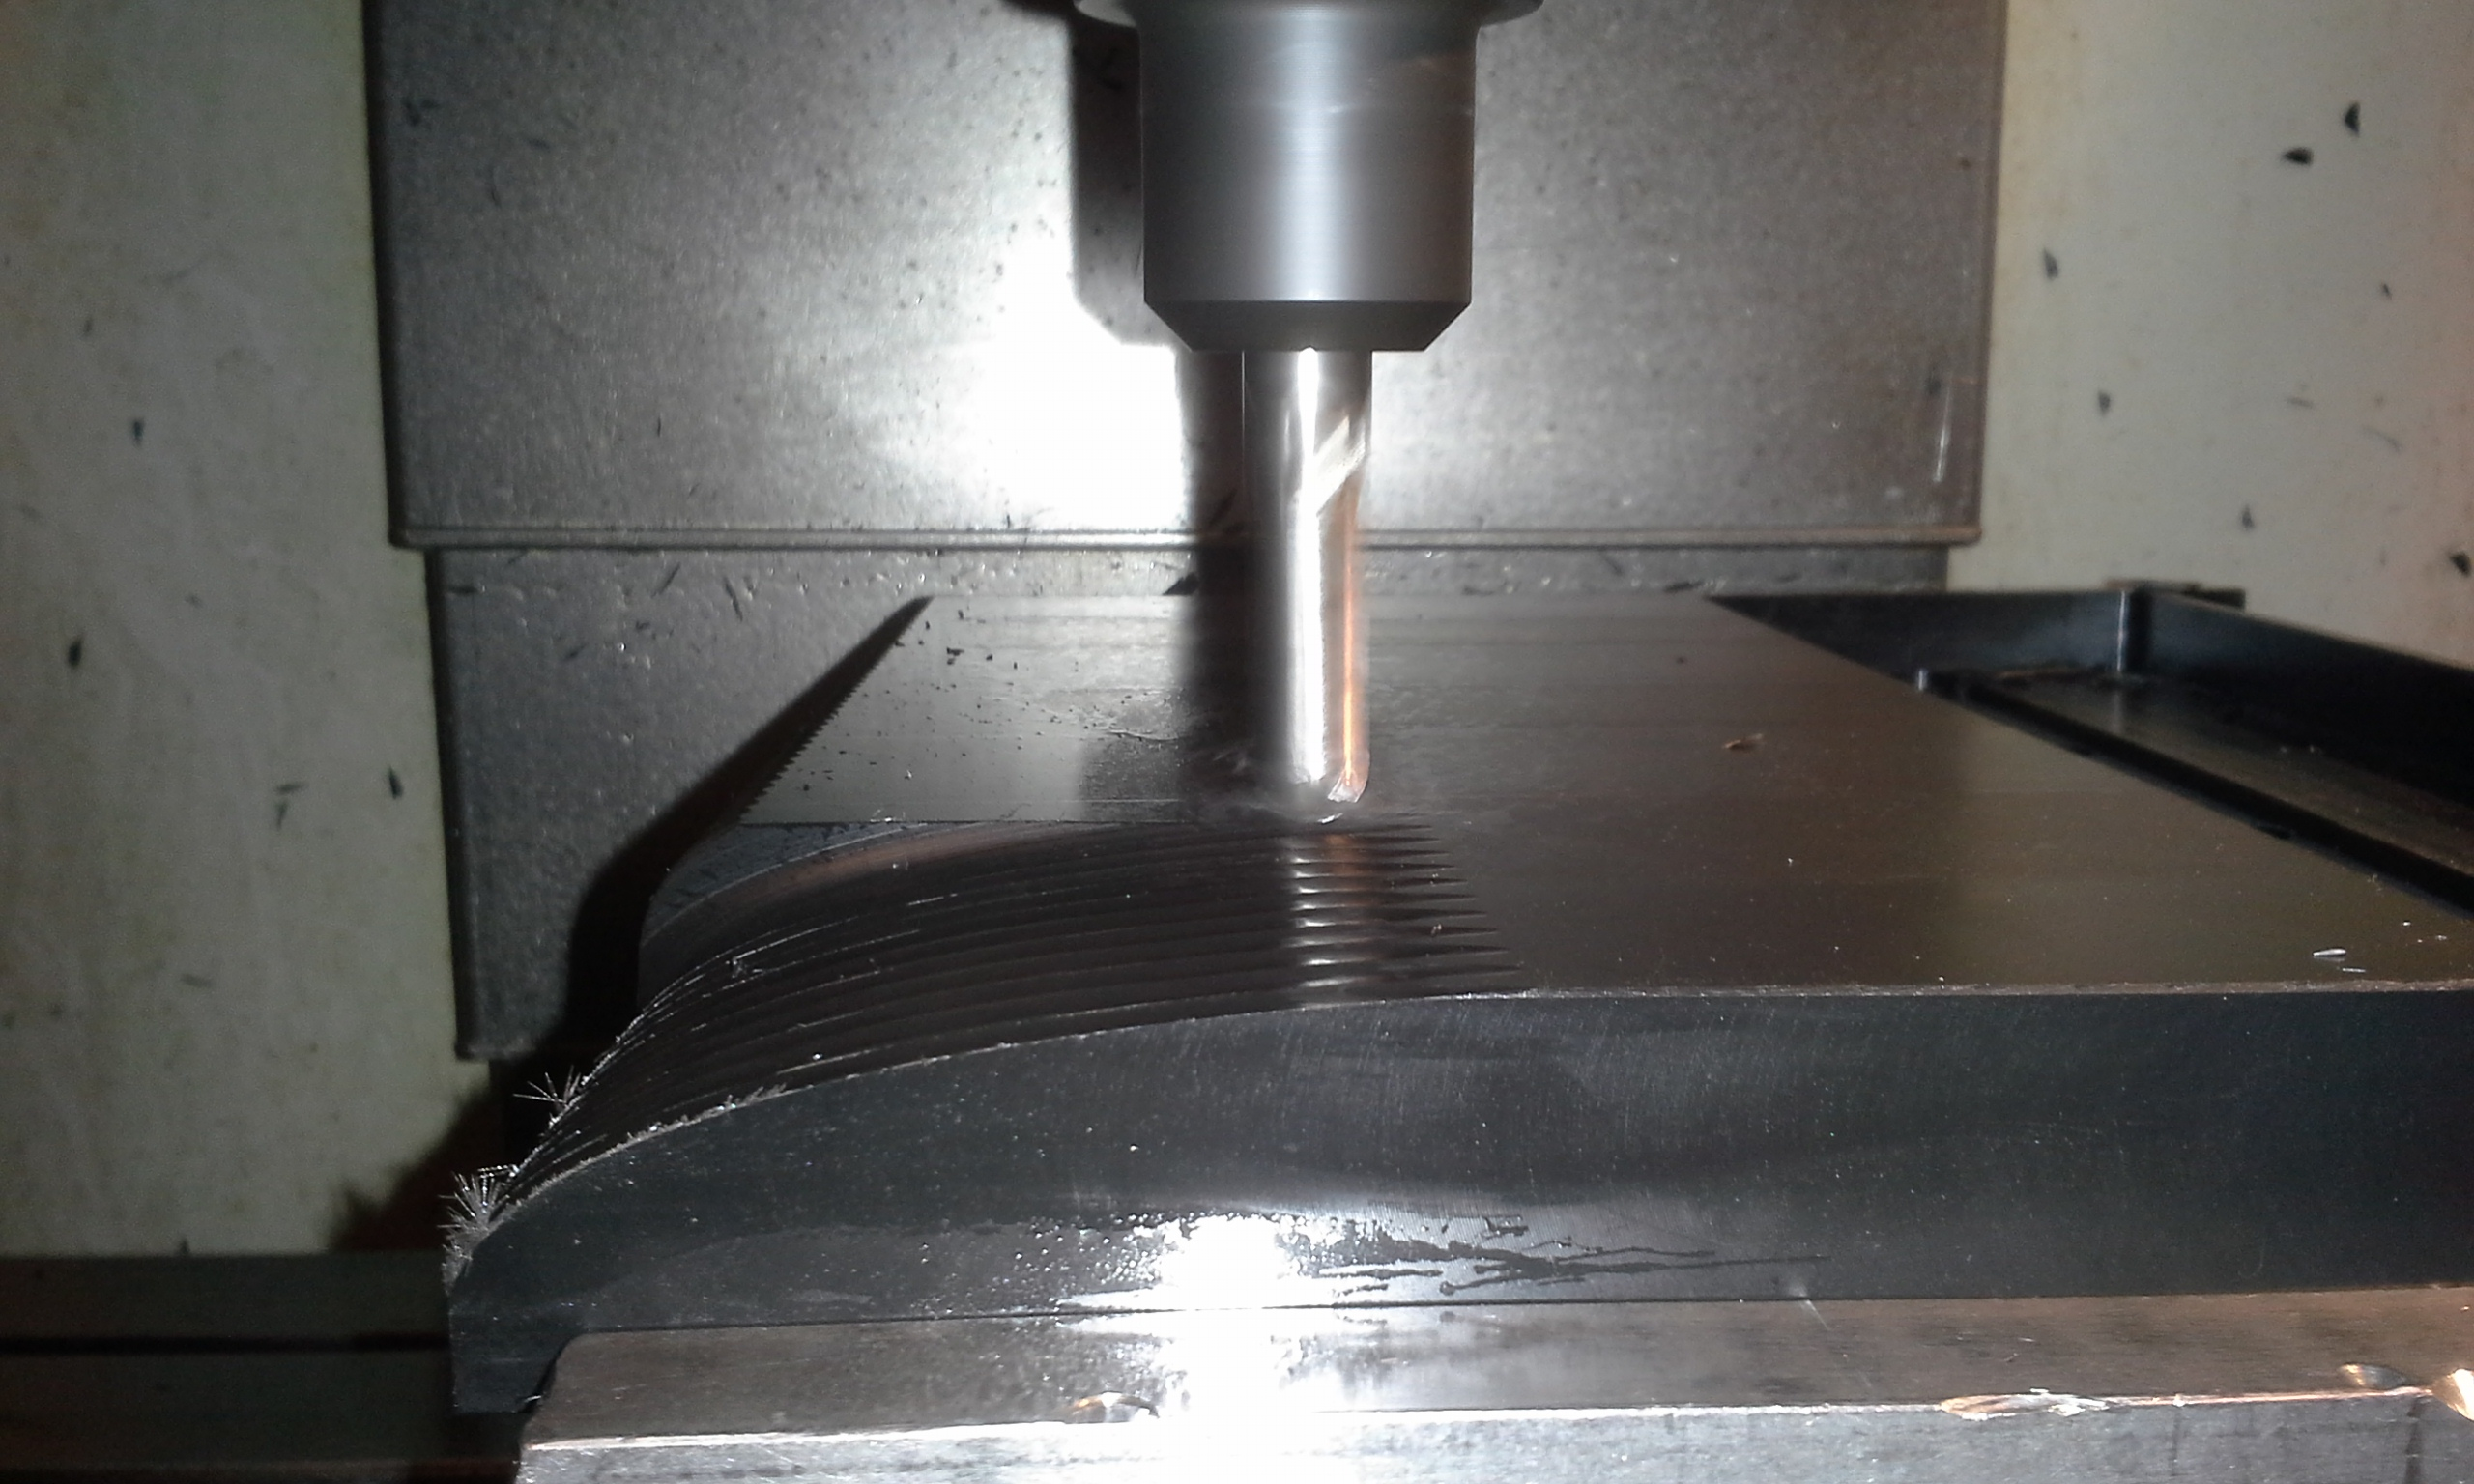
\includegraphics[scale=0.08]{facility/MachinedParts/noseMachine.jpg}}}
   {\subfigcapskip = 5pt \subfigcapmargin = -12pt  \subfigure[]{\label{fig:edge-b}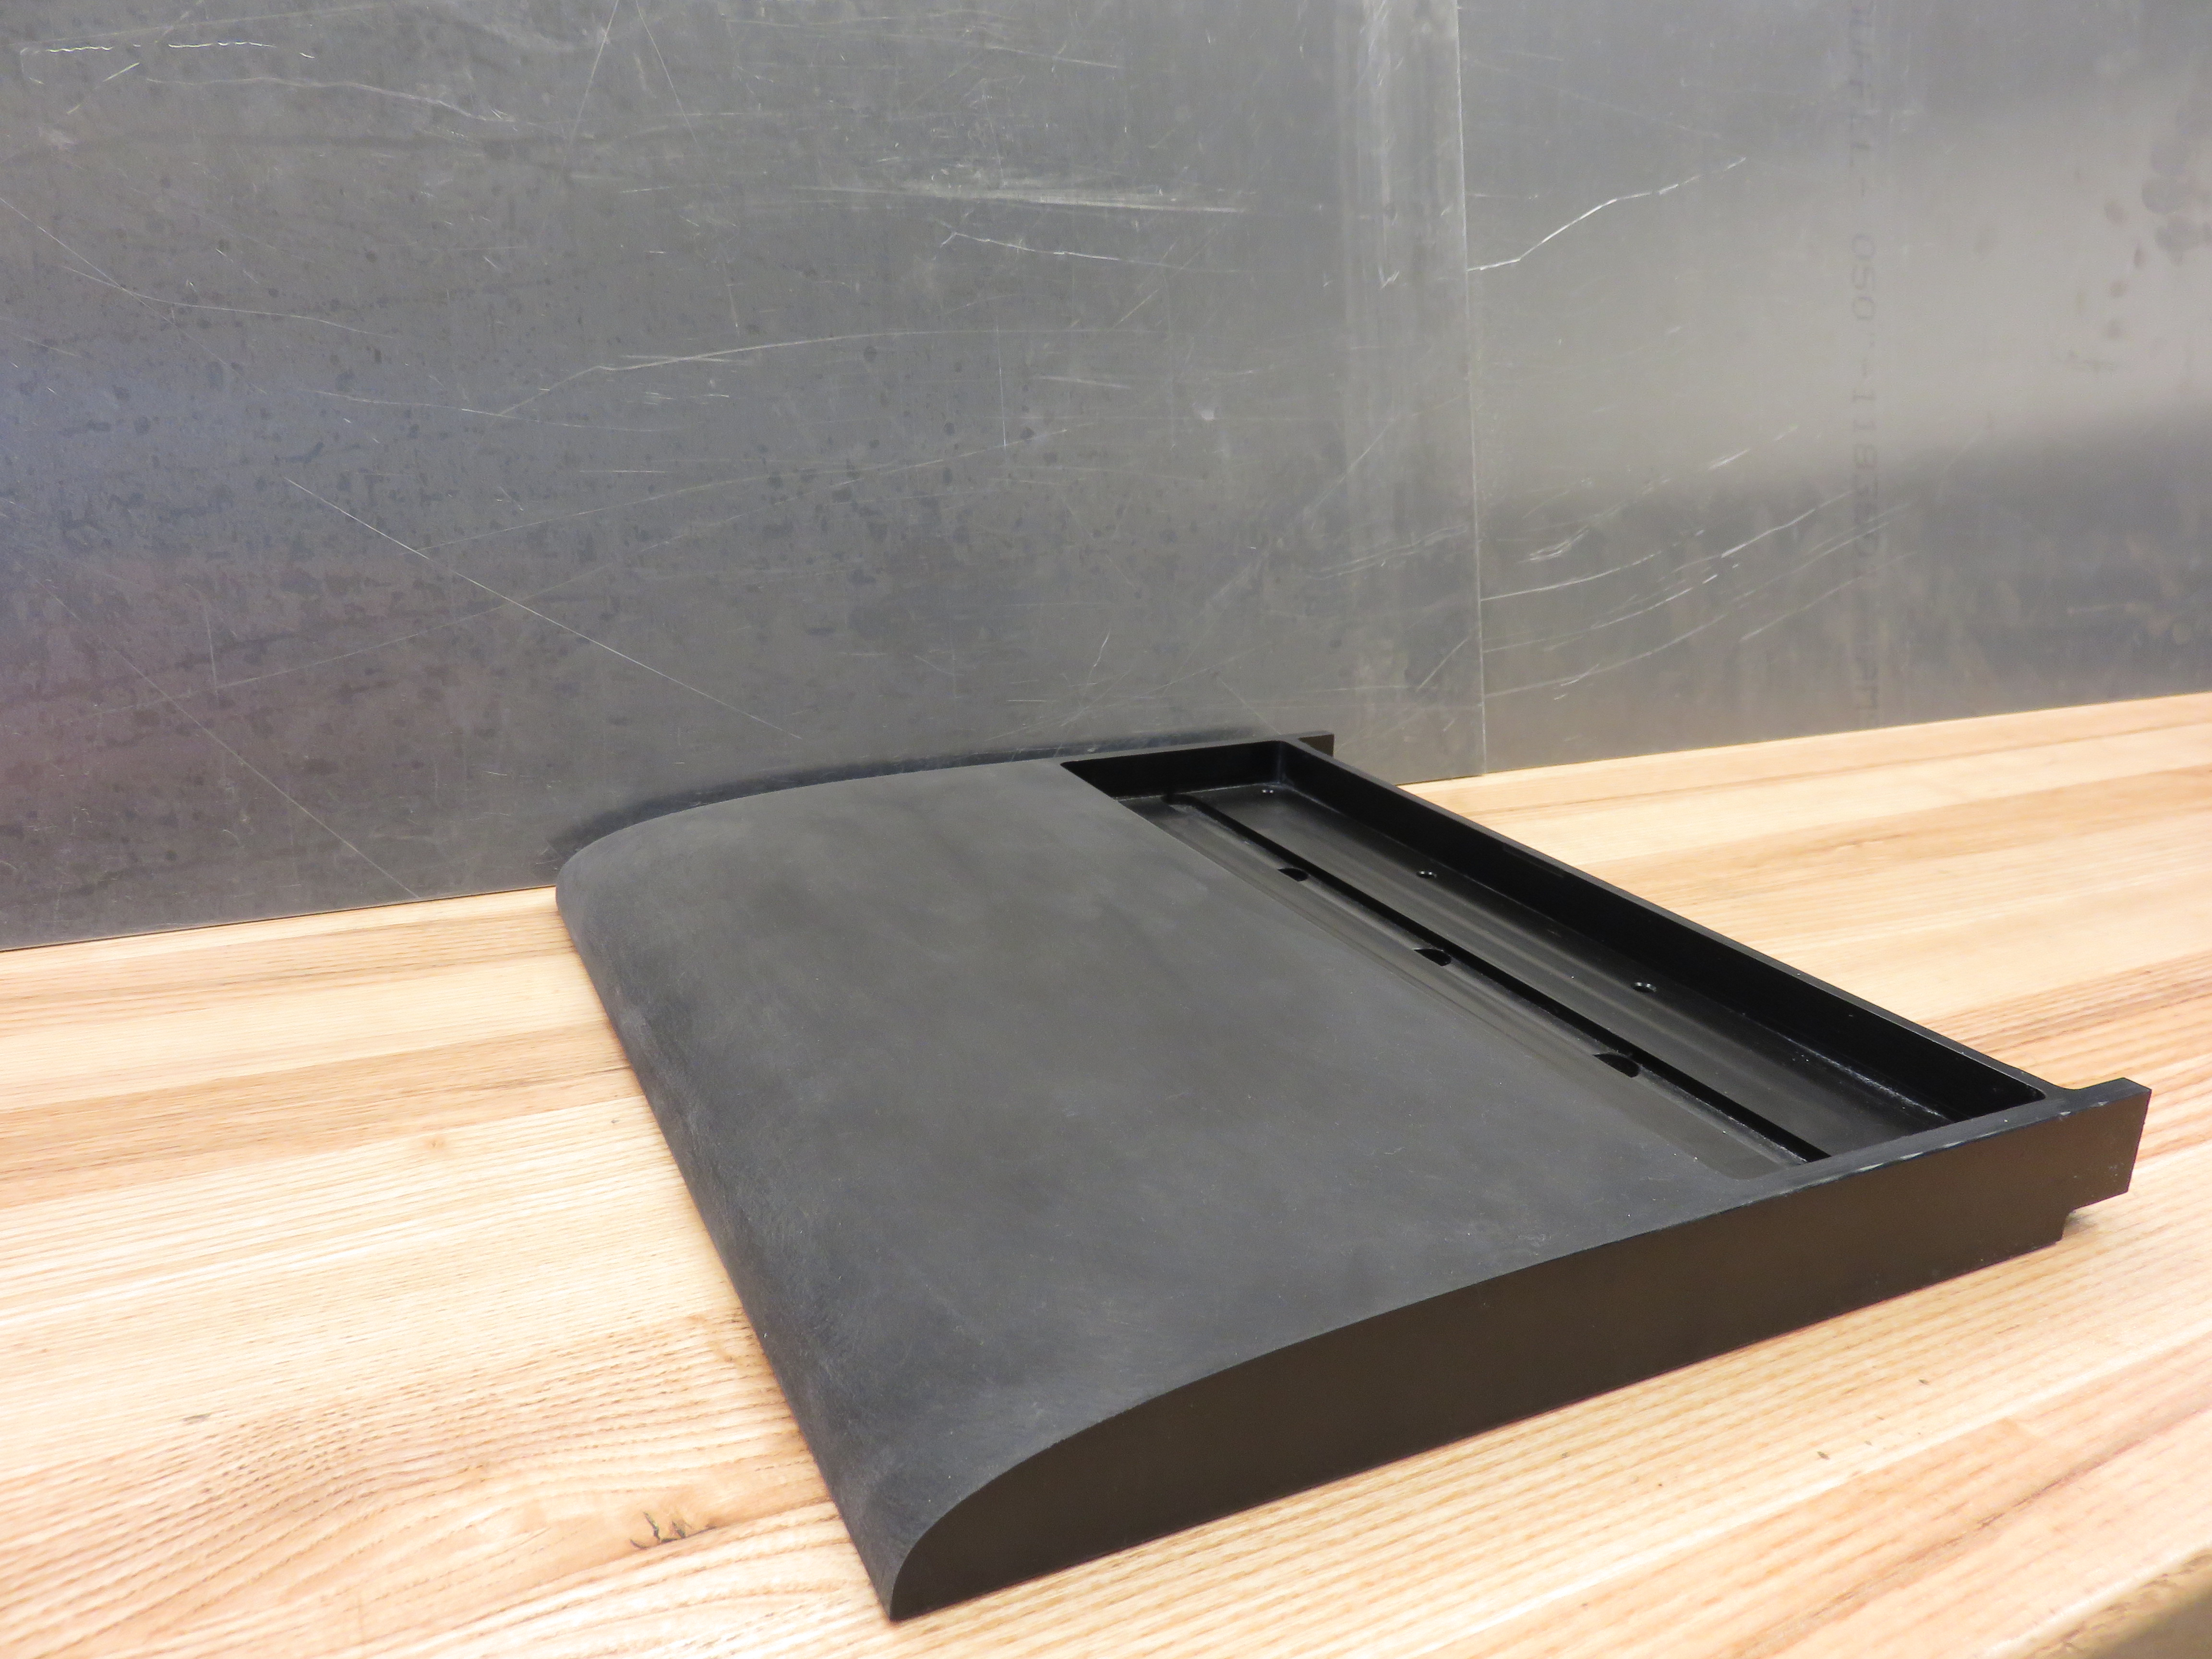
\includegraphics[scale=0.09]{facility/MachinedParts/A_v4.JPG}}}
  \end{center}
\caption{(a) Image of roughing pass for the fabrication of the super-ellipse leading edge nose of the wall plate (b) final image of leading edge frame component for the wall plate} 
\label{fig:nose}
\end{figure}

The temperature of each section of the thermal wall-plate is monitored and maintained by its own feedback controller as illustrated in Fig.~\ref{fig:tempcontrol}.  
LabVIEW is used to define and implement the controller settings. Each controller consists of a 10$A$ SCR and an NPN transistor. 
The average temperature of the three embedded thermocouples in each convective plate serves as the feedback parameter to direct the SCR to block/pass the 110 VAC that powers the resistive heaters (effectively the SCR serves as a switch to quickly turn the heaters on/off). 
The time constant of the controller is significantly smaller than the time constant of any given convective plate so the controller can monitor and adjust the heat-input to the convective plate much faster than the plate can lose (gain) heat to (from) the flow. 
The operating plate temperature range is 20$^\circ$C to 65$^\circ$C which is set by the working temperature of the materials used.
The controller is able to set and maintain a temperature of the system to within 0.5$^\circ$C as determined from the variance of the embedded thermocouples during testing. 
Details on the controller design and operation can be found in the thesis of Dr. Alireza Ebadi \cite{Ebadi2016}.
Importantly, since the temperature of each section of the thermal wall plate is independently controlled, the design allows for the application of a wide-range of thermal boundary conditions: e.g., isothermal, streamwise temperature gradient, discrete temperature steps, among others.

\begin{figure}[h!]
\centering
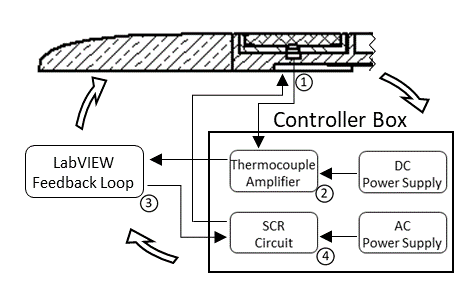
\includegraphics[scale=1]{figures/facility/circuit_diagram_v2.png}
\caption{{\footnotesize A diagram detailing the wall plate heater controller circuit. (1) designates the embedded thermocouples, which are fed to an amplifier (3), whose signal is then fed to a LabVIEW program (2), which determines if the heaters should be in an off or on position and sends a final signal to an SCR circuit (4), which communicates to the thermal wallplate heaters.
}}
\label{fig:tempcontrol}
\end{figure}

%%%%%%%%%%%%%%%%%%%%%%%%%%%%%%%%%%%%%%%
%%%%%%%%%%%%%%%%%%%%%%%%%%%%%%%%%%%%%%%%
\section{Pulsatile Flow Generator}
%discuss first design, outcomes and then second design
Pulsatile flows are periodic and unidirectional characterized by both their frequency and amplitude. 
The flow over a half-period first accelerates to maximum velocity then decelerates to the mean velocity. 
During the next half-period, the flow first decelerates to minimum velocity then accelerates to the mean velocity.
In a pulsatile boundary layer flow, the acceleration/deceleration of the freestream velocity  produces non-equilbrium flow behaviors. 
In particular, when the oscillation period is comparable to (or smaller than) the turbulence relaxation time (order $100 \nu / u_\tau^2$, \cite{Peters1993}), there will be a phase difference between the oscillating strain and stress field \cite{Weng2016}. 

\subsection{Rotor-Stator Assembly}
A rotor-stator assembly located downstream of the test-section was the first design used to generate a periodic pressure gradient used to produce a pulsatile freestream velocity in the tunnel. 
The design of the rotor-stator shown in Fig.~\ref{fig:rotor_stator}. is modeled after the design of K.Al-Asmi \textit{et al.} \cite{K.Al-Asmi1993}.
It consists of a rotor with 4 uniformly spaced holes, and a stator with 4 matching slots. 
The open area to the incoming flow is continuously modulated which produces a smooth sinusoidal freestream velocity signal as shown in Fig.~\ref{fig:rotor_stator}(c). 
The rotor frequency is controlled via a DC motor with variable speed settings from 1-100Hz. 
Twelve air-bleed slots arranged on the stator control the ratio of fluctuating area to open area. 
The slots ensure the existence of a mean flow and by changing the ratio of fluctuating area to mean through area the pulsatile flow amplitude can be adjusted. 
In the present design, this area ratio can be adjusted from 40$\%$ to 100$\%$. 
The rotor-stator assembly was mounted downstream of the test section to reduce the effect of induced rotational flow within the test-section. 
The assembly can be easily removed if a pulsatile flow is not desired.
 
\begin{figure}[t!]
\centering
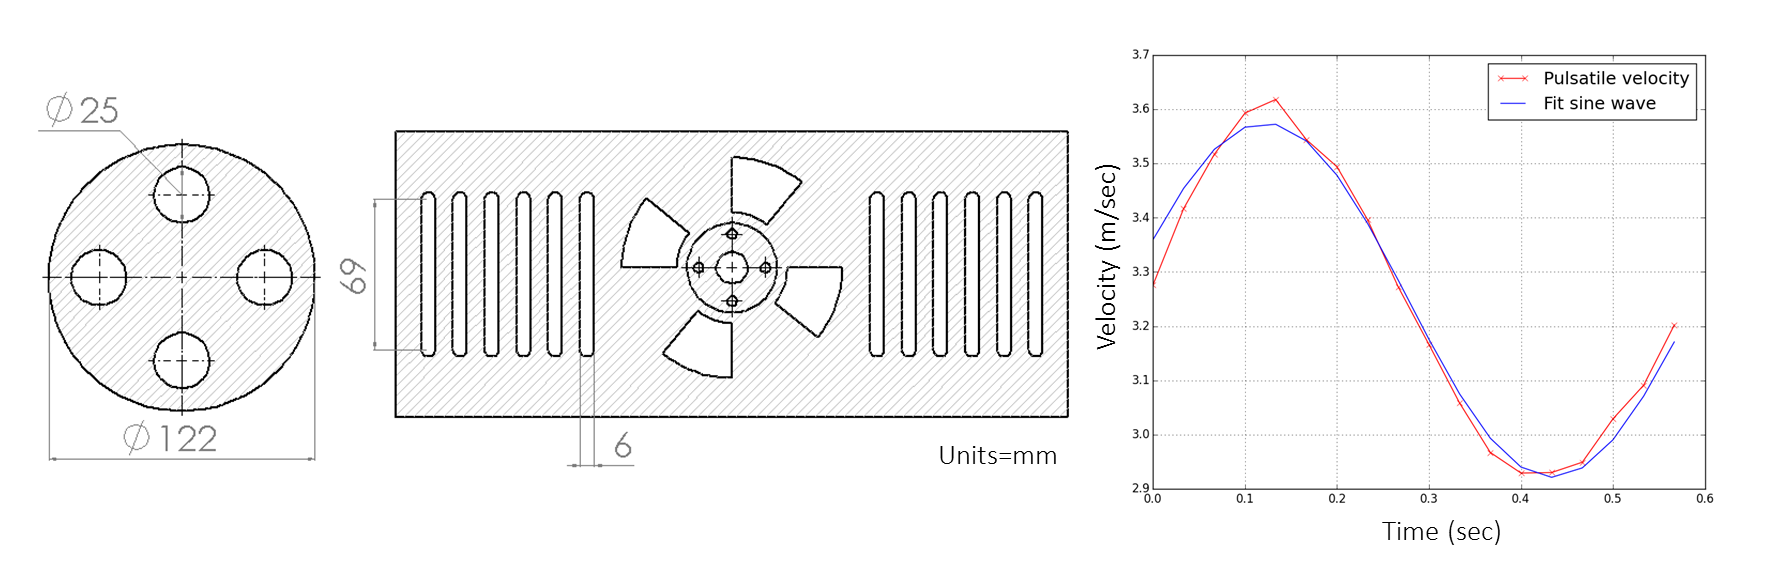
\includegraphics[scale=0.5]{facility/rotor_stator.png}
\caption{ \footnotesize Schematic of rotor-stator design, left shows the rotor, shown in the middle is the stator, and the right plot depicts a freestream velocity time series taken with a pitot-static tube for a quarter revolution of the rotor-stator mechanism.}
\label{fig:rotor_stator}
\end{figure}

%%%%%%%%%%%%%%%%%%%%%%%%%%%%%%%%%%%%%%
\subsection{Pulsatile Flow Generator}

\begin{figure}[h!]
\centering
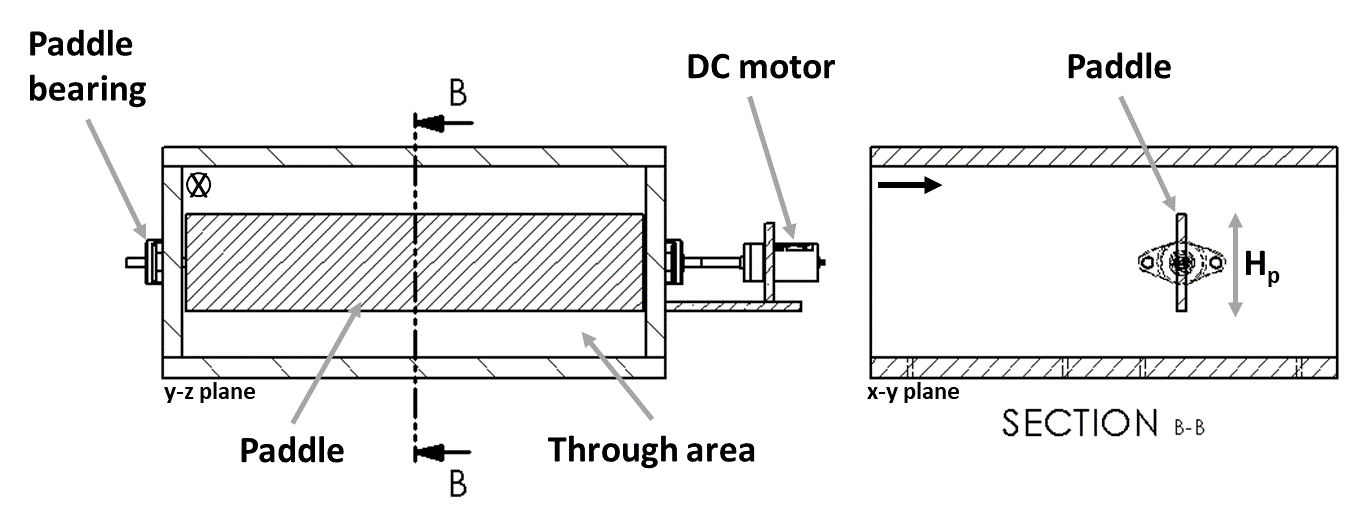
\includegraphics[scale=0.6]{facility/pulsatileGenV1.png}
\caption{ \footnotesize Schematic of pulsatile wave genorator with a paddle design. The left image displays the y-z plane with flow going into the paper, the right figure shows a cutaway image of the x-y plane on the tunnel centerline (B-B). The paddle height $H_p$ can be adjusted to change the fluctuating area and therefore the pulsatile amplitude.}
\label{fig:rotor_stator}
\end{figure}

The rotor-stator mechanism went through a re-design process due to the desire for a design with a lower blockage ratio which would then allow for testing of higher $Re$ flows.
In Karlsson \textit{et al.} a vertical array of spanwise orientated paddles were rotated to create a pulsatile pressure wave \cite{Karlsson1958}.
These paddles would create a similar sinusoidal change in through area yet drastically reduce the blockage ratio.
A similar design was developed to fit within the rotor-stator mechanism box which uses 1 paddle that mounts into bearings on each spanwise wall.
The paddle spans the entire width of the tunnel and connects to a DC gear motor {\bf (list exact motor)} that sits outside the tunnel and operates in a feeback loop with an Arduino.
Multiple paddles of varying heights can be installed to vary the fluctuating area.
The blockage ratio is reduced to 5\% and Re up to {\bf XX} can be reached.

